
% This LaTeX was auto-generated from an M-file by MATLAB.
% To make changes, update the M-file and republish this document.

\documentclass{article}
\usepackage{graphicx}
\usepackage{color}

\sloppy
\definecolor{lightgray}{gray}{0.5}
\setlength{\parindent}{0pt}

\begin{document}

    
    \begin{verbatim}
% Christian Sherland
% 2-14-13
% ECE411 - Speech Processing Project 1
%
%   Read all training set .wav files and
%   parse data appropriately so features
%   can be handled by HMM/ANN
%
%   Bugs:
%    1. Works. Small loss of data on first index
%       to fix 0 index problem.
%
%    2. Must be placed in the propper directory
%       before running
%

clear all;
clc;

%Get structures containing all pertinent file names
trainingSoundFiles = dir('../Datasets/Office Live/singlesounds_stereo/singlesounds_stereo/*.wav');
trainingSoundAnnot = dir('../Datasets/Office Live/singlesounds_annotation/Annotation2/*.txt');

ceps = zeros(length(trainingSoundFiles),13);
label = zeros(length(trainingSoundFiles),1);

%Read signals in one at a time
%and feed to hmm to avoid memory overflow
for ii = 1:length(trainingSoundFiles)
   %the iith signal
   [traData,fs] = wavread(strcat('../Datasets/Office Live/singlesounds_stereo/singlesounds_stereo/',trainingSoundFiles(ii).name));

   %the iith signal identification tag
   fid = fopen(strcat('../Datasets/Office Live/singlesounds_annotation/Annotation2/',trainingSoundAnnot(ii).name));
   traAnnot = textscan(fid,'%f%f','delimiter','\t');
   fclose(fid);

   %extracted signal and name of event
   pureTrainingSignal = traData(ceil(traAnnot{1}(1)*fs)+1:floor(traAnnot{2}(1)*fs)-1,1);
   trainingSignalLabel = trainingSoundAnnot(ii).name(1:find(isletter(trainingSoundAnnot(ii).name)==0,1,'first')-1);

   %Extract signal features here
   ceps(ii,:) = mean(mfcc(pureTrainingSignal,fs),2)';
   label(ii) = getClassNum(trainingSignalLabel);
end

%Generate training dataSet
trainingDataSet = prtDataSetClass(ceps,label);

%Read time tags for training set
fid = fopen('../Datasets/Office Live/events_OL_development/annotation1/script01_bdm.txt');
testDataLabelCell = textscan(fid,'%f%f%s','delimiter','\t');
fclose(fid);

%Read testing dataset sound file
[y,fs] = wavread('../Datasets/Office Live/events_OL_development/bformat/script01-01.wav');

actualSignals = {};     %eventually preallocate for efficiency
noise = {};
\end{verbatim}
\begin{verbatim}
%Parse testing data signals upon tags
for ii = 1 : length(testDataLabelCell{1})
   start = ceil(testDataLabelCell{1}(ii)*fs);
   finish = floor(testDataLabelCell{2}(ii)*fs);
   actualSignals{ii} = y(start:finish);

   start2 = floor(testDataLabelCell{2}(ii)*fs);
   startPad= [testDataLabelCell{1}; length(y)/fs];
   finish2= ceil(startPad(ii+1)*fs);

   noise{ii} = y(start2:finish2);
end
\end{verbatim}
\begin{verbatim}
subplot(2,1,1)
plot(noise{1})
subplot(2,1,2)
plot(actualSignals{1})
\end{verbatim}

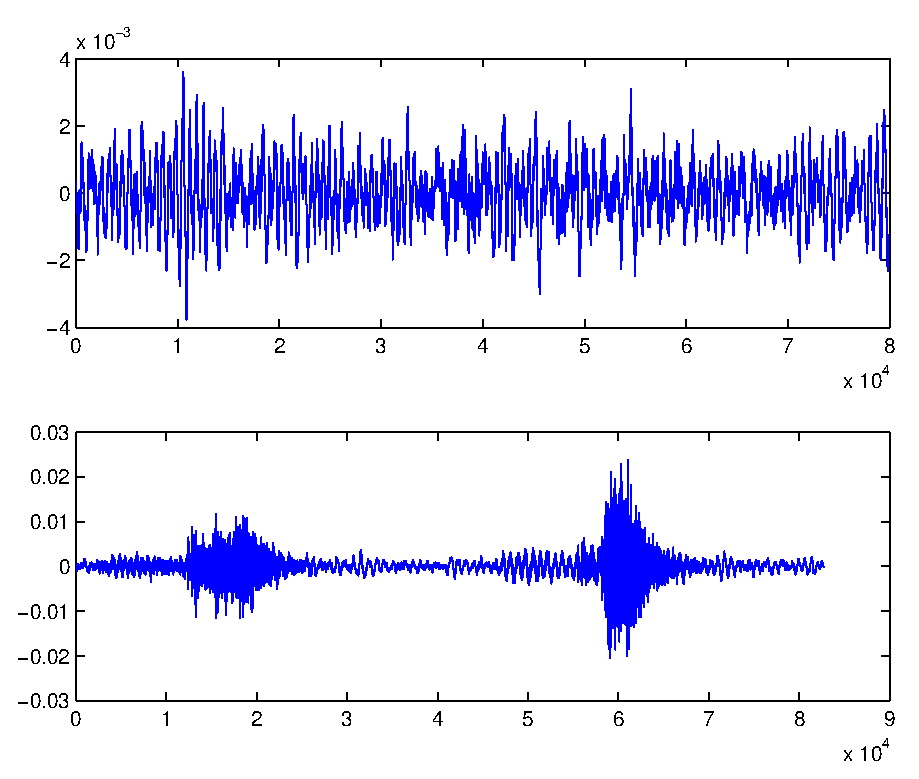
\includegraphics [width=4in]{readTrainingData_01.eps}
\begin{verbatim}
%remake ceps and label for test dataSet
ceps = zeros(numel(actualSignals),13);
label = zeros(numel(testDataLabelCell{3}),1);

%Determine relavant features for each signal.
for ii = 1 : numel(actualSignals)
    ceps(ii,:) = mean(mfcc(actualSignals{ii},fs),2)';
    label(ii) = getClassNum(testDataLabelCell{3}(ii));
end

%Generate test dataSet
testingDataSet = prtDataSetClass(ceps,label);

classifier = prtClassBinaryToMaryOneVsAll;   % Create a classifier
classifier.baseClassifier = prtClassGlrt;    % Set the binary

% Set the internal Decider
classifier.internalDecider = prtDecisionMap;

classifier = classifier.train(trainingDataSet);   % Train
classes    = run(classifier, testingDataSet);     % Test

% Evaluate, plot results
percentCorr = prtScorePercentCorrect(classes.getX,testingDataSet.getTargets);
\end{verbatim}



\end{document}
    
